\documentclass[runningheads]{llncs}

\usepackage[T1]{fontenc}
\usepackage{hyperref}
\usepackage{color}
\renewcommand\UrlFont{\color{blue}\rmfamily}
\urlstyle{rm}
\usepackage{graphicx}
\usepackage{amsmath}
\usepackage{amssymb}
\usepackage{tikz}
\usetikzlibrary{positioning,arrows.meta,fit,backgrounds}
\usepackage[ruled,vlined]{algorithm2e}
\usepackage{fixme}
\fxsetup{draft}

\allowdisplaybreaks

\newcommand{\rGB}{\textsc{$r$-GB} }
\newcommand{\rGBP}{$r$-GBP }

\makeatletter
\AtBeginDocument{%
	\renewcommand\doi[1]{}%
}
\makeatother

\begin{document}
	
	\title{AI-driven Diversification for De Novo Enzyme Discovery}
	\author{}
	\institute{}
	\maketitle
	
	%=================================================================
	\section{Introduction and Motivation}
	
	The AIZyme project aims to develop a computational pipeline for the \emph{de novo} generation of enzymatic structures capable of reproducing catalytic functionality while exploring previously unknown regions of protein structure space. Existing protein engineering approaches are largely limited to modifying known enzymes, leaving most of the theoretical protein fold space unexplored. We hypothesize that modern generative AI models can be combined with structural prediction tools and machine learning–based analysis to systematically explore this manifold and identify candidates that preserve catalytic geometry while exhibiting structural diversity.
	
	%=================================================================
	\section{AI-driven Workflow for Diversified Enzyme Discovery}
	
	The proposed workflow consists of tightly coupled stages designed to generate, evaluate, and diversify candidate enzyme structures before experimental validation. The overall objective is to explore a broader region of the structural design space while preserving key catalytic motifs, increasing the probability of discovering novel enzyme scaffolds with improved or entirely new catalytic capabilities.
	
	\subsection{Generative Structural Exploration}
	
	Candidate backbones are generated using diffusion-based protein generative models~\cite{yim2024diffusion}, enforcing geometric constraints from reference enzymes. For each backbone, multiple sequences are predicted with \texttt{ProteinMPNN}~\cite{dauparas2022robust}. These sequences are evaluated using \texttt{AlphaFold}~\cite{jumper2020alphafold}, providing 3D coordinates and confidence metrics (pLDDT, PAE).
	
	\subsection{Structural Validation and Functional Preservation}
	
	Global similarity (RMSD) and catalytic site descriptors (geometry, pocket volume) ensure functional preservation. Candidates failing to reproduce key catalytic motifs are discarded.
	
	\subsection{Graph-based Structural Representation and Feature Extraction}
	
	Structures are converted to spatial graphs (residues = nodes; edges = proximity/interactions). Graph-based descriptors include centrality, density, radius, minimum dominating set size~\cite{nacher2016minimum,milenkovic2011dominating}, and maximum quasi-cliques~\cite{bhattacharyya2009mining}. Metaheuristic algorithms~\cite{lin2016effective,pullan2011cooperating} compute these features efficiently, tuned using \texttt{Optuna}~\cite{agrawal2020optuna}, executed in parallel on the VEGA HPC cluster.
	
	Feature vectors $x_s \in \mathbb{R}^d$ capture multi-dimensional structural and topological properties for downstream analysis.
	
	\subsection{Diversity-aware Clustering}
	
	Unsupervised clustering (e.g., $k$-means, hierarchical clustering) partitions candidate structures~\cite{zou2020sequence}. Representative structures from each cluster are sampled to maintain diversity, while discarded structures are replaced via new generative cycles. This iterative loop ensures exploration of multiple structural regions.
	
	\subsection{Adaptive Diversification via AI-guided Feedback}
	
	Three AI strategies guide exploration:
	
	\begin{enumerate}
		\item \textbf{AlphaFold-based diversification:} Low pLDDT regions are targeted for structural variation.
		\item \textbf{Graph Neural Network scoring:} Predicts stability and catalytic potential from residue interaction graphs.
		\item \textbf{Active learning loop:} Experimental results refine predictive models and guide the next generation of candidates.
	\end{enumerate}
	
	%=================================================================
\begin{figure}[t]
	\centering
	\scalebox{0.7}{
	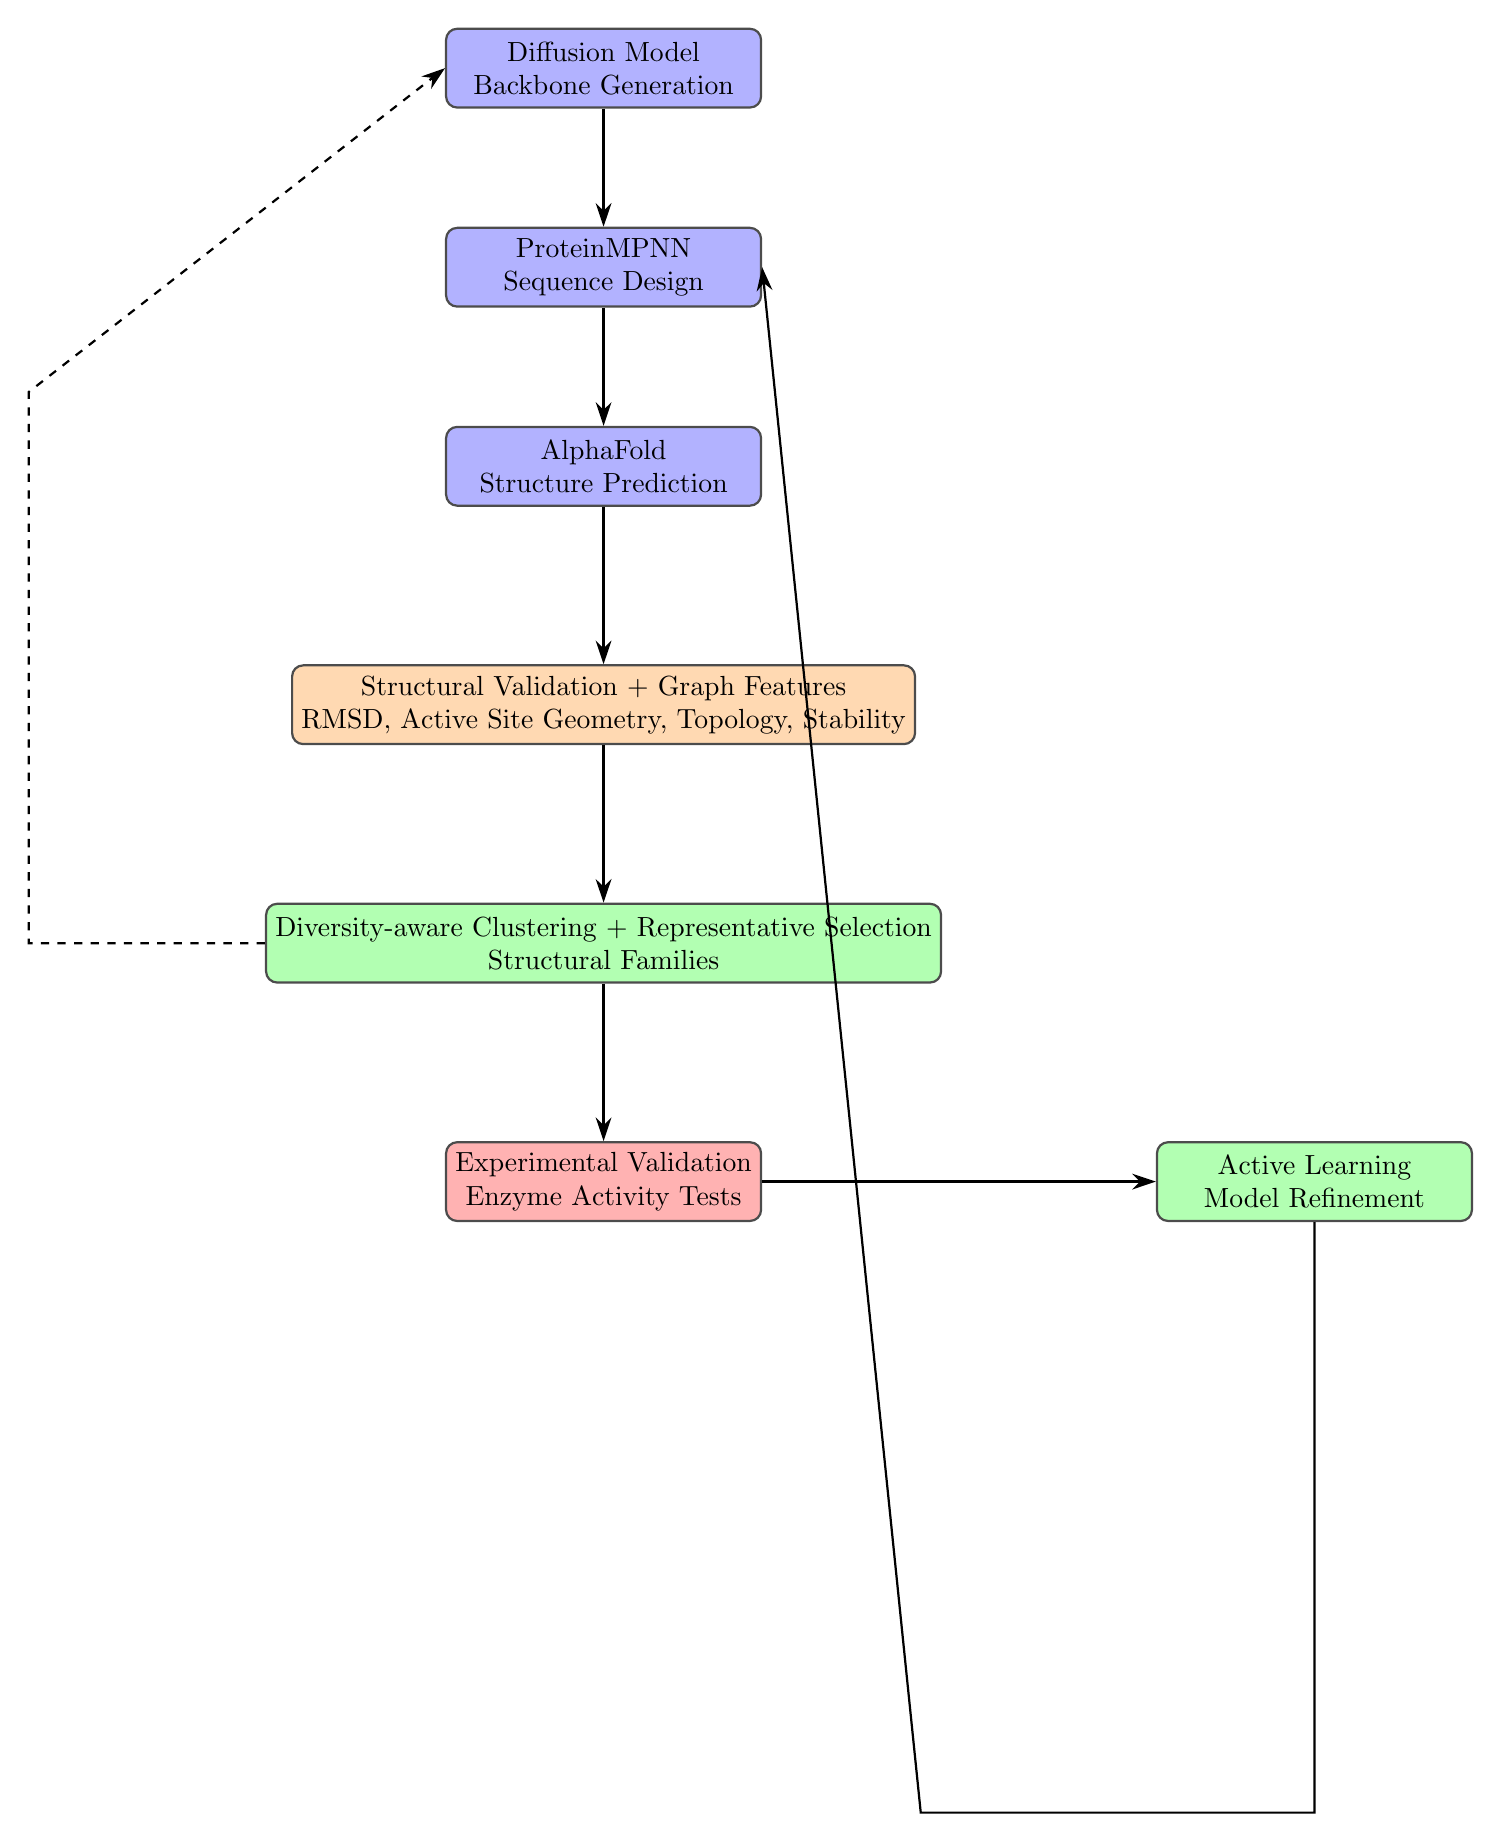
\begin{tikzpicture}[
		node distance=2cm,
		stage/.style={rectangle, draw=black!70, fill=#1!30, thick, minimum width=4cm, minimum height=1cm, align=center, rounded corners},
		arrow/.style={-{Stealth[length=3mm, width=2mm]}, thick}
		]
		
		%==================== Nodes ====================%
		\node[stage=blue] (diffusion) {Diffusion Model \\ Backbone Generation};
		\node[stage=blue, below=1.5cm of diffusion] (mpnn) {ProteinMPNN \\ Sequence Design};
		\node[stage=blue, below=1.5cm of mpnn] (alphafold) {AlphaFold \\ Structure Prediction};
		
		\node[stage=orange, below=2cm of alphafold] (analysis) {Structural Validation + Graph Features \\ RMSD, Active Site Geometry, Topology, Stability};
		
		\node[stage=green, below=2cm of analysis] (clustering) {Diversity-aware Clustering + Representative Selection \\ Structural Families};
		
		\node[stage=red, below=2cm of clustering] (lab) {Experimental Validation \\ Enzyme Activity Tests};
		
		\node[stage=green, right=5cm of lab] (active) {Active Learning \\ Model Refinement};
		
		%==================== Arrows ====================%
		\draw[arrow] (diffusion) -- (mpnn);
		\draw[arrow] (mpnn) -- (alphafold);
		\draw[arrow] (alphafold) -- (analysis);
		\draw[arrow] (analysis) -- (clustering);
		\draw[arrow] (clustering) -- (lab);
		
		\draw[arrow] (lab.east) -- ++(2,0) -- (active.west);
		\draw[arrow] (active.south) -- ++(0,-7.5) -- ++(-5.0,0) -- (mpnn.east);
		
		% Optional dashed feedback for diversification
		\draw[arrow, dashed] (clustering.west) -- ++(-3,0) -- ++(0,7) -- (diffusion.west);
		
	\end{tikzpicture}}
	\caption{Simplified AI-driven workflow for diversified de novo enzyme discovery. Core stages include generative backbone modeling, sequence design, structure prediction, structural validation with graph-based features, diversity-aware clustering, and experimental validation. Active learning feedback loops enable iterative improvement of candidate enzymes.}
\end{figure}
	%=================================================================
	\section{Research Questions and Objectives}
	
	\textbf{Research Questions:}
	
	\begin{itemize}
		\item RQ1: Can generative AI explore protein structures inaccessible via natural evolution?
		\item RQ2: How can structural diversity be quantified and actively enforced during enzyme design?
		\item RQ3: Can graph-based descriptors reveal structural families with catalytic potential?
		\item RQ4: Do AI-generated scaffolds preserve native catalytic geometry?
		\item RQ5: Can iterative AI–lab feedback progressively improve enzyme discovery?
	\end{itemize}
	
	\textbf{Objectives:}
	
	\begin{itemize}
		\item O1: Diffusion-based exploration of protein fold space.
		\item O2: Diversity-aware sequence and structure generation.
		\item O3: Graph-based feature extraction for stability and catalytic potential.
		\item O4: AI-guided clustering and candidate selection.
		\item O5: Closed-loop AI–experimental validation for progressive improvement.
	\end{itemize}
	
	%=================================================================
	\section{Scientific Impact}
	
	AIZyme targets a transformative approach to enzyme discovery beyond naturally evolved proteins. Immediate impact includes enzymes for PET degradation and environmental applications. Long-term impact encompasses:
	
	\begin{itemize}
		\item Autonomous discovery of enzymes for green chemistry and sustainable synthesis,
		\item Design of biocatalysts for industrial biotechnology,
		\item Creation of novel metabolic pathways in synthetic biology,
		\item Establishment of a paradigm-shifting AI-driven enzyme discovery platform.
	\end{itemize}
	
	%=================================================================
	\begin{thebibliography}{99}
		
		\bibitem{jumper2020alphafold}
		J. Jumper et al.,
		``AlphaFold 2,''
		\textit{Fourteenth Critical Assessment of Techniques for Protein Structure Prediction}, vol. 13, DeepMind, London, UK, 2020.
		
		\bibitem{dauparas2022robust}
		J. Dauparas et al.,
		``Robust deep learning--based protein sequence design using ProteinMPNN,''
		\textit{Science}, vol. 378, no. 6615, pp. 49--56, 2022.
		
		\bibitem{yim2024diffusion}
		J. Yim et al.,
		``Diffusion models in protein structure and docking,''
		\textit{Wiley Interdisciplinary Reviews: Computational Molecular Science}, vol. 14, no. 2, p. e1711, 2024.
		
		\bibitem{djukanovic2019beam}
		M. Djukanovic et al.,
		``A beam search for the longest common subsequence problem guided by a novel approximate expected length calculation,''
		in \textit{Proc. Int. Conf. on Machine Learning, Optimization, and Data Science}, pp. 154--167, Springer, 2019.
		
		\bibitem{lin2002longest}
		G. Lin et al.,
		``The longest common subsequence problem for sequences with nested arc annotations,''
		\textit{J. Comp. \& System Sciences}, vol. 65, no. 3, pp. 465--480, 2002.
		
		\bibitem{castelli2017longest}
		M. Castelli et al.,
		``The longest filled common subsequence problem,''
		in \textit{Proc. 28th Annual Symposium on Combinatorial Pattern Matching}, Schloss Dagstuhl, 2017.
		
		\bibitem{chen2011generalized}
		Y.-C. Chen, K.-M. Chao,
		``On the generalized trained longest common subsequence problems,''
		\textit{J. Combinatorial Optimization}, vol. 21, no. 3, pp. 383--392, 2011.
		
		\bibitem{katoh2008recent}
		K. Katoh, H. Toh,
		``Recent developments in the MAFFT multiple sequence alignment program,''
		\textit{Briefings in Bioinformatics}, vol. 9, no. 4, pp. 286--298, 2008.
		
		\bibitem{chatzou2016multiple}
		M. Chatzou et al.,
		``Multiple sequence alignment modeling: methods and applications,''
		\textit{Briefings in Bioinformatics}, vol. 17, no. 6, pp. 1009--1023, 2016.
		
		\bibitem{nacher2016minimum}
		J. C. Nacher, T. Akutsu,
		``Minimum dominating set-based methods for analyzing biological networks,''
		\textit{Methods}, vol. 102, pp. 57--63, 2016.
		
		\bibitem{milenkovic2011dominating}
		T. Milenković et al.,
		``Dominating biological networks,''
		\textit{PLoS ONE}, vol. 6, no. 8, p. e23016, 2011.
		
		\bibitem{bhattacharyya2009mining}
		M. Bhattacharyya, S. Bandyopadhyay,
		``Mining the largest quasi-clique in human protein interactome,''
		in \textit{Proc. 2009 Int. Conf. on Adaptive and Intelligent Systems}, IEEE, 2009.
		
		\bibitem{lin2016effective}
		G. Lin et al.,
		``An effective hybrid memetic algorithm for the minimum weight dominating set problem,''
		\textit{IEEE Trans. Evol. Comput.}, vol. 20, no. 6, pp. 892--907, 2016.
		
		\bibitem{pullan2011cooperating}
		W. Pullan et al.,
		``Cooperating local search for the maximum clique problem,''
		\textit{J. Heuristics}, vol. 17, no. 2, pp. 181--199, 2011.
		
		\bibitem{zou2020sequence}
		Q. Zou et al.,
		``Sequence clustering in bioinformatics: an empirical study,''
		\textit{Briefings in Bioinformatics}, vol. 21, no. 1, pp. 1--10, 2020.
		
		\bibitem{agrawal2020optuna}
		T. Agrawal,
		``Optuna and AutoML,''
		in \textit{Hyperparameter Optimization in Machine Learning}, Springer, pp. 109--129, 2020.
		
	\end{thebibliography}
	
\end{document}